\documentclass{article}
\usepackage[a4paper, margin=3mm, landscape]{geometry}
\usepackage{multicol}
\usepackage{xcolor}
\usepackage{enumitem}
\usepackage{amsmath}
\usepackage{amsfonts}
\usepackage{listings}
\usepackage{soul}
\usepackage{graphicx}

\pdfinfo{
    /Title (GEC1010.pdf)
    /Creator (TeX)
    /Producer (pdfTeX 1.40.0)
    /Author (Vincent Pang)
    /Subject (GEC1010)
    /Keywords (GEC1010, nus, cheatsheet, pdf)
}

\graphicspath{ {./img/} }

\pagestyle{empty}
\setcounter{secnumdepth}{0}
\setlength{\columnseprule}{0.25pt}

% Redefine section commands to use less space
\makeatletter
\renewcommand{\section}{\@startsection{section}{1}{0mm}%
    {-1ex plus -.5ex minus -.2ex}%
    {0.5ex plus .2ex}%x
{\normalfont\large\bfseries}}
\renewcommand{\subsection}{\@startsection{subsection}{2}{0mm}%
    {-1explus -.5ex minus -.2ex}%
    {0.5ex plus .2ex}%
{\normalfont\normalsize\bfseries}}
\renewcommand{\subsubsection}{\@startsection{subsubsection}{3}{0mm}%
    {-1ex plus -.5ex minus -.2ex}%
    {1ex plus .2ex}%
{\normalfont\small\bfseries}}%
\makeatother

% Adjust spacing for all itemize/enumerate
\setlength{\leftmargini}{0.5cm}
\setlength{\leftmarginii}{0.5cm}
\setlist[itemize,1]{leftmargin=2mm,labelindent=1mm,labelsep=1mm}
\setlist[itemize,2]{leftmargin=2mm,labelindent=1mm,labelsep=1mm}

% Font
\renewcommand{\familydefault}{\sfdefault}

% Define colors for math formulas
\definecolor{myblue}{cmyk}{1,.72,0,.38}
\everymath\expandafter{\the\everymath \color{myblue}}

% Custom command for keywords
\definecolor{highlight}{RGB}{251,243,218}
\newcommand{\keyword}[2][]{\sethlcolor{highlight}\hl{\textbf{#2}} #1 - }
\newcommand{\ilkeyword}[1]{\sethlcolor{highlight}\hl{\textbf{#1}}}

% Define colors and style for code
\definecolor{codegreen}{rgb}{0,0.6,0}
\definecolor{codegray}{rgb}{0.5,0.5,0.5}
\definecolor{codered}{HTML}{CC241D}
\definecolor{backcolor}{rgb}{0.95,0.95,0.95}
\lstdefinestyle{codestyle}{
    backgroundcolor = \color{backcolor},
    commentstyle = \color{codegray},
    keywordstyle = \color{codered},
    stringstyle = \color{codegreen},
    basicstyle = \ttfamily,
    breakatwhitespace = false,
    showstringspaces = false,
    breaklines = true,
    showtabs = false,
    tabsize = 2
}
\lstset{style = codestyle}

% -----------------------------------------------------------------------
\begin{document}
\begin{multicols*}{3}
\footnotesize

% Title box
\begin{center}
    \fbox{
        \parbox{0.8\linewidth}{
            \centering \textcolor{black}{
                {\Large\textbf{GEC1010}} \\
                \normalsize{AY22/23 Sem 2}} \\
                {\footnotesize \textcolor{gray}{github.com/securespider}}
        }
    }
\end{center}
\section{05. Hydro power}
\subsection{Ocean vs River}
River
\begin{enumerate}
	\item Hydroelectricity
\end{enumerate}
Ocean
\begin{enumerate}
	\item Tidal power
	\item Wave power
	\item Ocean thermal
\end{enumerate}
\subsection{Water wheels}
\subsubsection{Water mills}
\begin{itemize}
	\item Ancient application for replacing physical labour
	\item Replaced with water turbines for energy generation
\end{itemize}
Types of water wheels\\
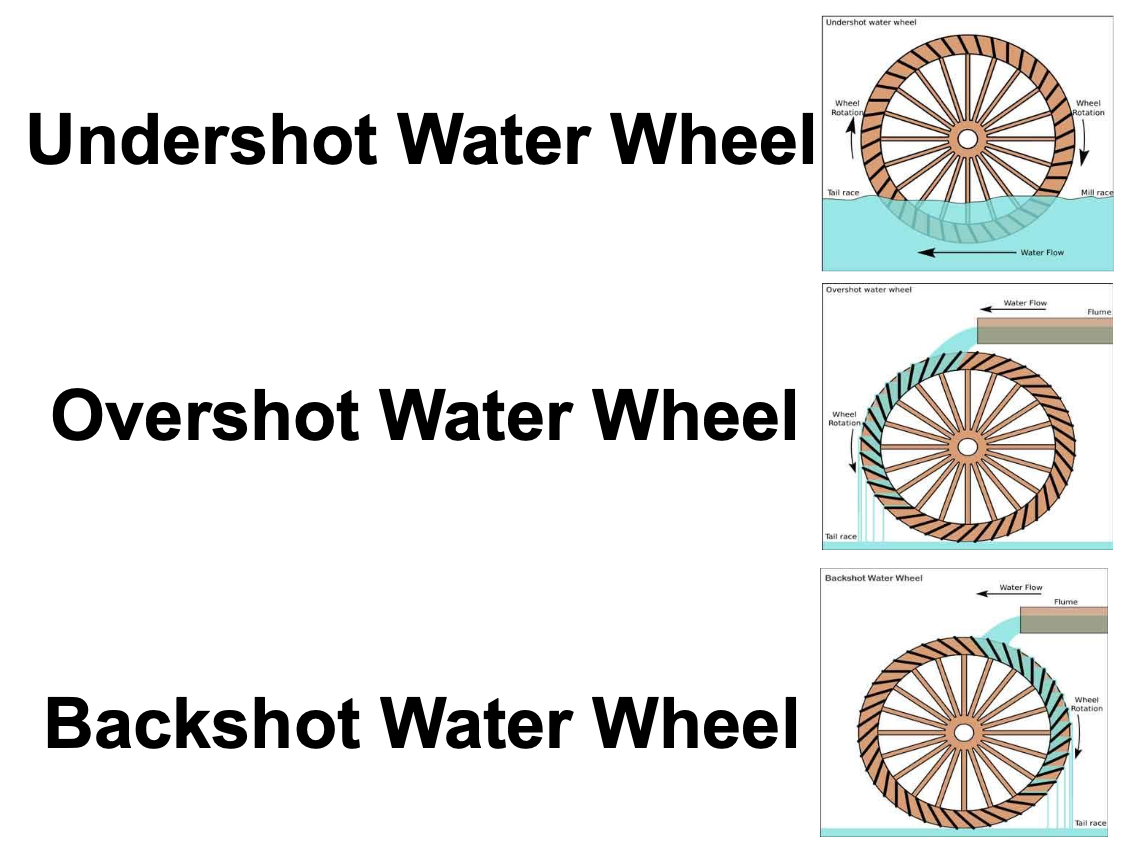
\includegraphics[scale=0.3]{water-wheels}
\begin{itemize}
	\item Undershot
	\begin{itemize}
		\item Vertically mounted with water flowing at the bottom of the wheel
		\item Cheapest and least efficient
	\end{itemize}
	\item Overshot
	\begin{itemize}
		\item Falling water on the top of the wheel in direction of rotation
		\item Use all water flow for power production 
		\item Does not require rapid flow of water
		\item Uses the difference in weight between the 2 sides of the wheel to turn
	\end{itemize}
	\item Backshot
	\begin{itemize}
		\item Introduced behind the apex of the wheel
		\item Water flows opposite the direction of rotation
		\item Continues to function even when water in wheel put rises beyond height of axle
		\item Technique useful for streams that experience extreme seasonal variations in flow
	\end{itemize}
\end{itemize}

\subsection{Types of Hydro Power}
\begin{itemize}
	\item Dam based
	\item Run of the river plants(diversion)
	\item Pumped storage technology
	\item Damless hydro power
\end{itemize}
\subsubsection{Principles of power generation}
Production of electricity by using gravitational force of falling water\\
$P=\eta\rho ghQ$\\
$\eta$ = efficiency, $\rho$ = density of water, Q = Volume of water flowing per second on turbine, h = Vertical distance between turbine and water surface

\end{multicols*}
\end{document}
